\doublespacing
\chapter{Introduction}
An ordered labeled tree is a tree in which the nodes are labeled and the left-to-right order among siblings is significant. One way of comparing two ordered labeled tree is by measuring their edit distance. 

Tree edit distance was first introduced by Tai~\cite{tai1979tree} as a generalization of the string editing problem. The computation of the string edit distance counts the minimum number of operations(insert, delete and replace) required to transform one string into the other, which quantifies the similarity between two strings. Similarly, given two ordered labeled tree $T_1$ and $T_2$, the tree edit distance between $T_1$ and $T_2$ is the minimum cost to transform one tree into another using three elementary operations: insert, delete and substitution. Tai gave an algorithm with a time complexity of $\mathcal{O}(\left\vert T_1 \right\vert^3 * \left\vert T_2 \right\vert^3)$. Later on, a number of improved algorithms were developed[~\cite{zhang1989simple}, ~\cite{klein1998computing}, ~\cite{dulucq2005decomposition}, ~\cite{demaine2009optimal}, ~\cite{Chen2014}, ~\cite{pawlik2015efficient}].

An ordered labeled tree can represent a scene description, an XML document, a natural language parse, and other phenomena. Given a pattern data and match data, we can formulate these data into two order labeled trees and we may want to match the pattern tree to the data tree.

RNA secondary structure comparison is an application of the tree edit distance. RNA is a single strand of nucleotides. The nucleotides in the strand have selectively sticky ends. Because of the stickiness, the strand bends around and sticks to itself, which is topologically a tree. This tree-like structure of RNA is called the secondary structure of RNA and is depicted in Figure 1.1. 

\begin{figure}
		\centering
		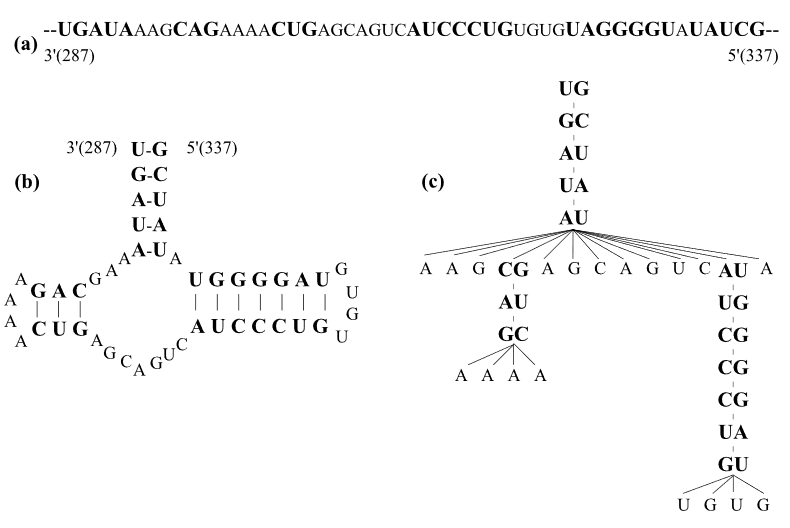
\includegraphics[width=14cm,clip]{Figures/RNATreeRepresentation}
		\label{RNA structures and forest representation} 
		\caption{RNA structures and forest representation. From ~\cite{Liang2012} (a) A segment of the RNA GI: 2347024 primary structure, (b) its secondary structure, (c) its forest representation}. 
\end{figure}

The secondary structure of RNA plays an important role in its functions preforming. In biology, it is presumed that a preserved biological function corresponds to a preserved molecular structure. Therefore, the comparison secondary structures of RNA is required in many biology problems with RNA involving, which helps reveal information regarding RNA functions.

We designed and implemented a new space and time efficient algorithm to compute the tree edit distance. Compared to other currently existing algorithm, the new algorithm use the best decomposition strategy for trees, which creates the least number of the relevant sub-problems. 

The thesis is organized as follows. Chapter 2 introduces the tree edit distance problem and the related work of tree edit distance algorithm. A number of related path decomposition algorithms are described in this chapter. A detailed explanation of the design and implementation of our improved algorithm follows in Chapter 3.Besides, another algorithmic improvement is introduced in Chapter 4. The evaluation of the new method is performed in Chapter 5 by comparing it with other leading methods and we conclude in Chapter 6.
